\chapter{Introduction}
\label{ch:introduction}

\section{Problem Approach}
In this section the approach to resolve the planning problem is described. For the table clearing task the main actions the robots has to use in order to interact with the objects are:
\begin{itemize}
\item Grasping
\item Pushing
\end{itemize}
Grasping is the most important action since it lets to take an object from the pile of objects and drop it somewhere, for example in a bin, clearing in this way the table. There exist different works facing the same task by focusing only in grasping. The planning becomes useful considering the problem that two adjacent objects could not be grasped if they are so close such that the robot's gripper, when attempting to grasp an object is going to collide with the other object, making such an object ungraspable. From this consideration is necessary the pushing action, in order to separate adjacent objects which mutually exclude themselves to be grasped.  And in order to face the problem in elegant way a planning system is used, instead of a heuristic approach for the action decision making stage.

\section{Set Up}
In order to make the understanding of the approach used the name the set up of the environment the robot will work in is presented. 
The robot used is a Barret WAM arm, which is a 7 degree of freedom (DoF) manipulator arm shown in Figure \ref{fig:wam_1}. 

This robot is characterized by a low inertia of the end effector thanks to the kind of its actuators. The WAM is noteworthy because it does not use any gears for manipulating the joints, but rather a cable drive, so there are no backlash problems and it is both fast and stiff. Cable drives permit low friction and ripple-free torque transmission from the actuator to the joints. 

\begin{figure}[htp]
\centering
\begin{subfigure}[b]{0.45\textwidth}
\centering
\includegraphics[height=5cm]{Img/set_up/wam.jpg}
\caption{Barrett WAM arm}\label{fig:wam_1}
\end{subfigure}
\begin{subfigure}[b]{0.45\textwidth}
\centering
\includegraphics[width=5cm]{Img/set_up/Kinect.jpg}
\caption{Microsoft Kinect sensor}\label{fig:wam_1}
\end{subfigure}
\caption{Robot and vision sensor.}
\end{figure}


To manipulate the objects the manipulation skills of the robot are enhanced by a gripper designed in the IRI institute driven by Dynamixel motors. Such a gripper is depicted in Figure \ref{fig:gripper_general} from several point of view. 

\begin{figure}[htp]
\centering
\begin{subfigure}[b]{0.3\textwidth}
\centering
\includegraphics[height=3cm]{Img/set_up/gripper1.png}
%\caption{}
\end{subfigure}
\begin{subfigure}[b]{0.3\textwidth}
\centering
\includegraphics[height=3cm]{Img/set_up/gripper2.png}
%\caption{}
\end{subfigure}
\begin{subfigure}[b]{0.3\textwidth}
\centering
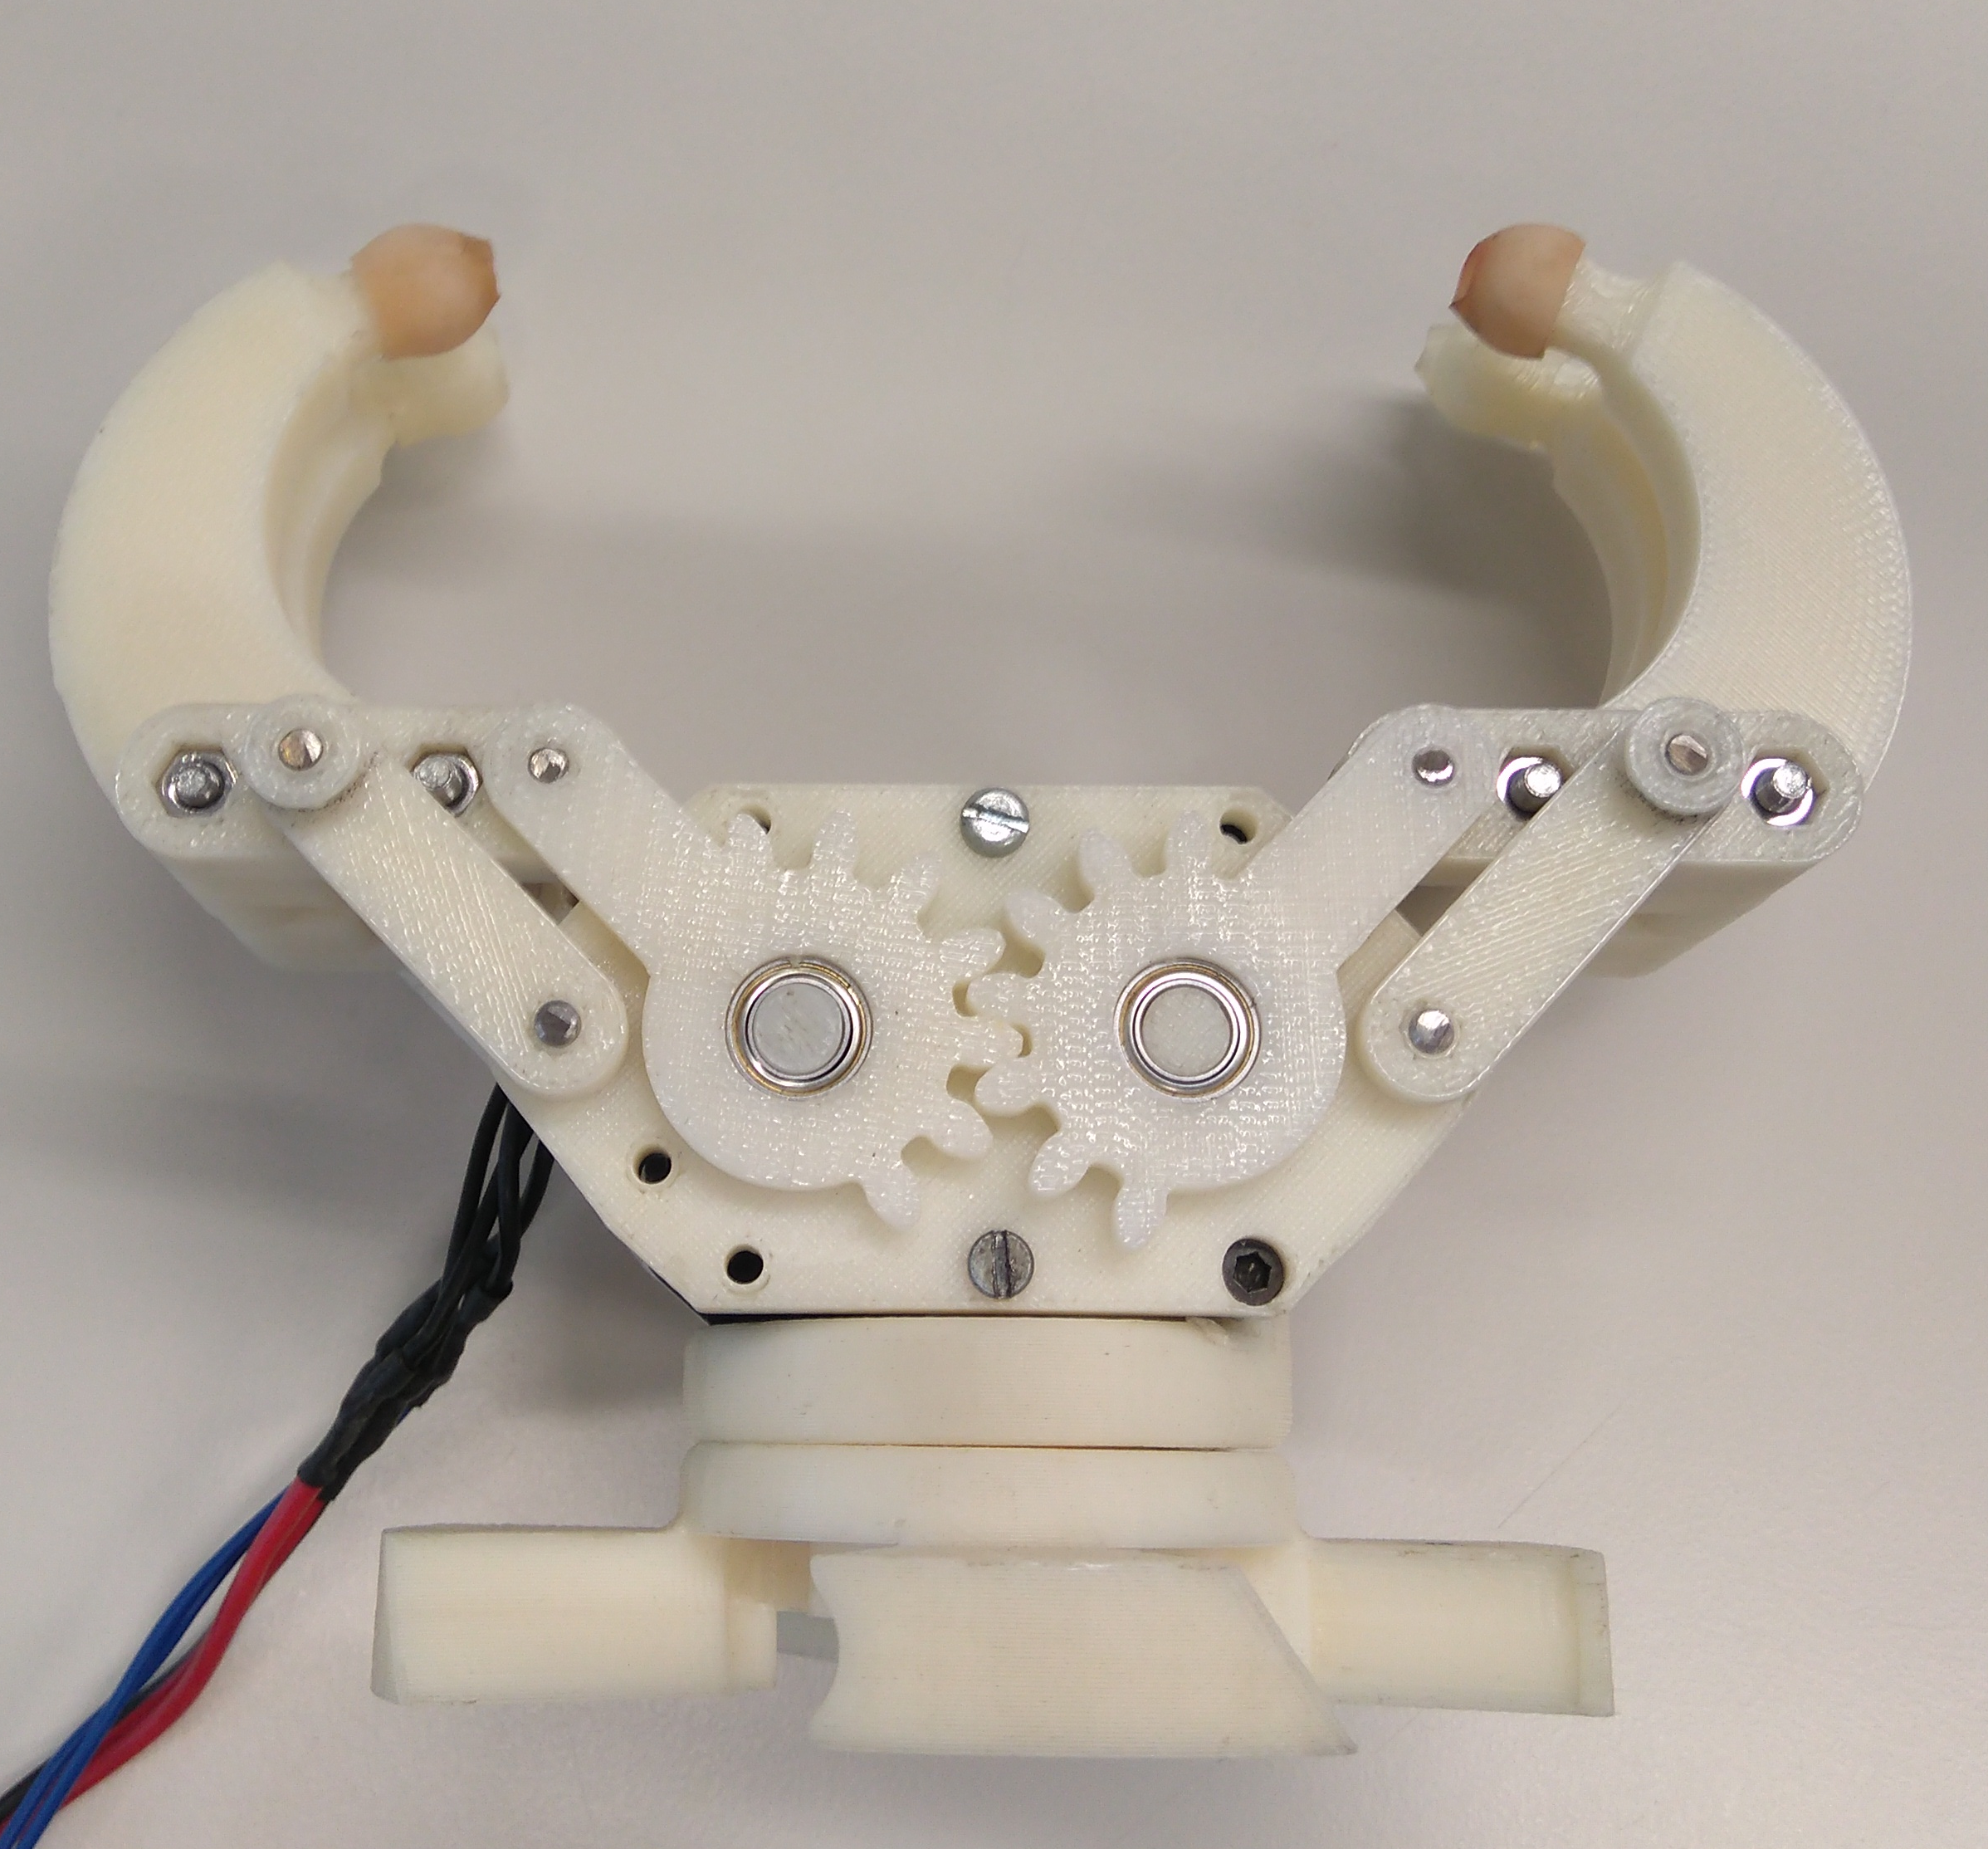
\includegraphics[width=3cm]{Img/set_up/gripper3.png}
%\caption{}
\end{subfigure}
\caption{Gripper used for the experiments}\label{fig:gripper_general}
\end{figure}

The gripper will be modelled measuring some principal elements such as: finger's width and height, gripper's width, height and deep, and the distance between the fingers when the gripper is opened or closed. The modelling procedure is depicted in Figure \ref{fig:gripper_modelling}. The resulting model is a simple polygonal mesh which includes all the important geometric information of the gripper.
\begin{wrapfigure}{r}{6.5cm}
\caption{Gripper and WAM.}\label{fig:wam_gripper}
\includegraphics[width=6.5cm]{Img/set_up/wam_gripper.png}
\end{wrapfigure}
Such a simple model allows to the collision algorithm commented in chapter \ref{ch:algorithm} in just few second. 
Having a more detailed and complex model would not lead any benefits but it will slow down the process. The model of the gripper will be an important resource for the task planner as the reader will see in chapters \ref{ch:task_planner} and \ref{ch:algorithm}.
The gripper will be mounted in the end effector of the robot as shown in Figure \ref{fig:wam_gripper}. 


\begin{figure}[htp]
\centering
\begin{subfigure}[t]{0.5\textwidth}
\centering
\stackunder[5pt]	{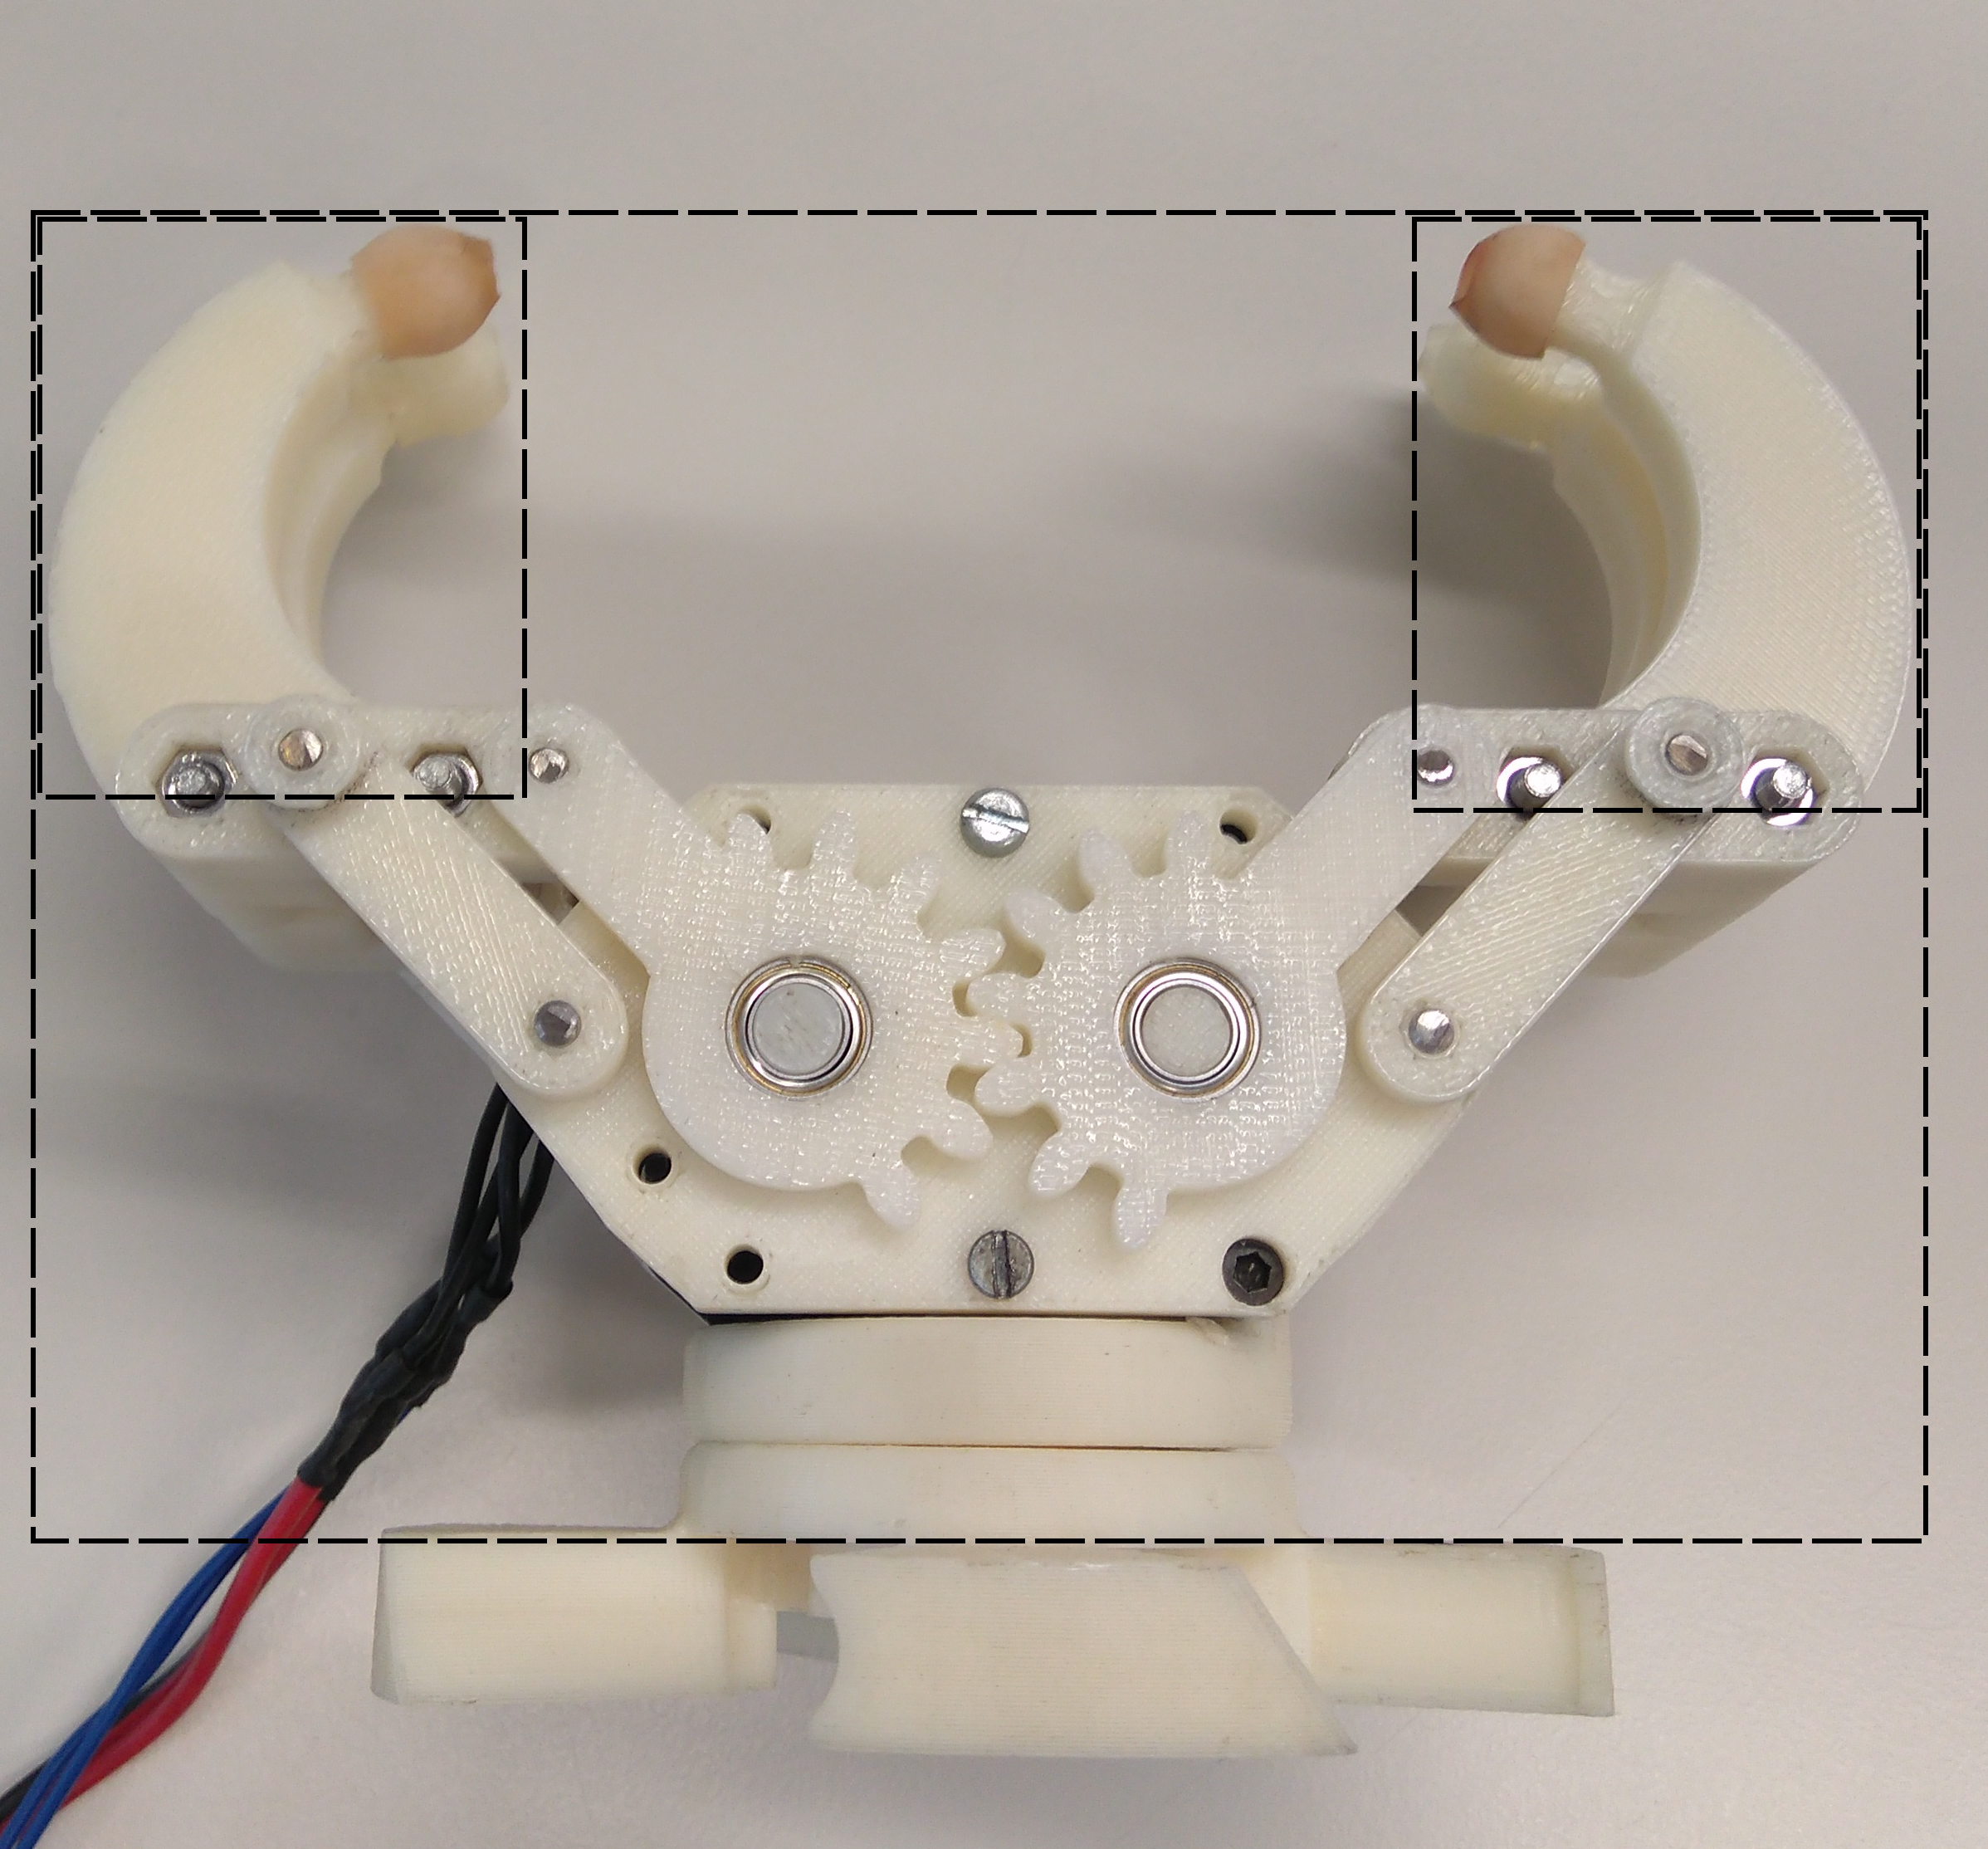
\includegraphics[height=4.5cm]{Img/set_up/gripper_modelling1.png}}{Elements measured}
\end{subfigure} \\
\begin{subfigure}[t]{0.3\textwidth}
\centering
\stackunder[5pt]	{\includegraphics[height=3cm]{Img/set_up/gripper_open_model.png}}{Opened gripper mesh model}
\end{subfigure}
\hspace{3cm}
\begin{subfigure}[t]{0.3\textwidth}
\centering
\stackunder[5pt]	{\includegraphics[height=3cm]{Img/set_up/gripper_closed_model.png}}{Closed gripper mesh model}
%\caption{}
\end{subfigure}
\caption{Modelling of the gripper: the fingers width, fingers height, the height of the whole gripper, its width and its deep have been measured. The \textcolor{red}{red}, \textcolor{green}{green} and \textcolor{blue}{blue} axis are respectively the x, y and z axis.}\label{fig:gripper_modelling}
\end{figure}

The scenario the robot is going to work in is presented by a table, and the objects will lay on top of it. The WAM arm is in a fixed position with respect the table and a Kinect sensor is located on top of the table pointing down. An example of the kinect view is, and an example of the scenario the robot is going to deal with is.. 

\begin{figure}[htp]
\centering
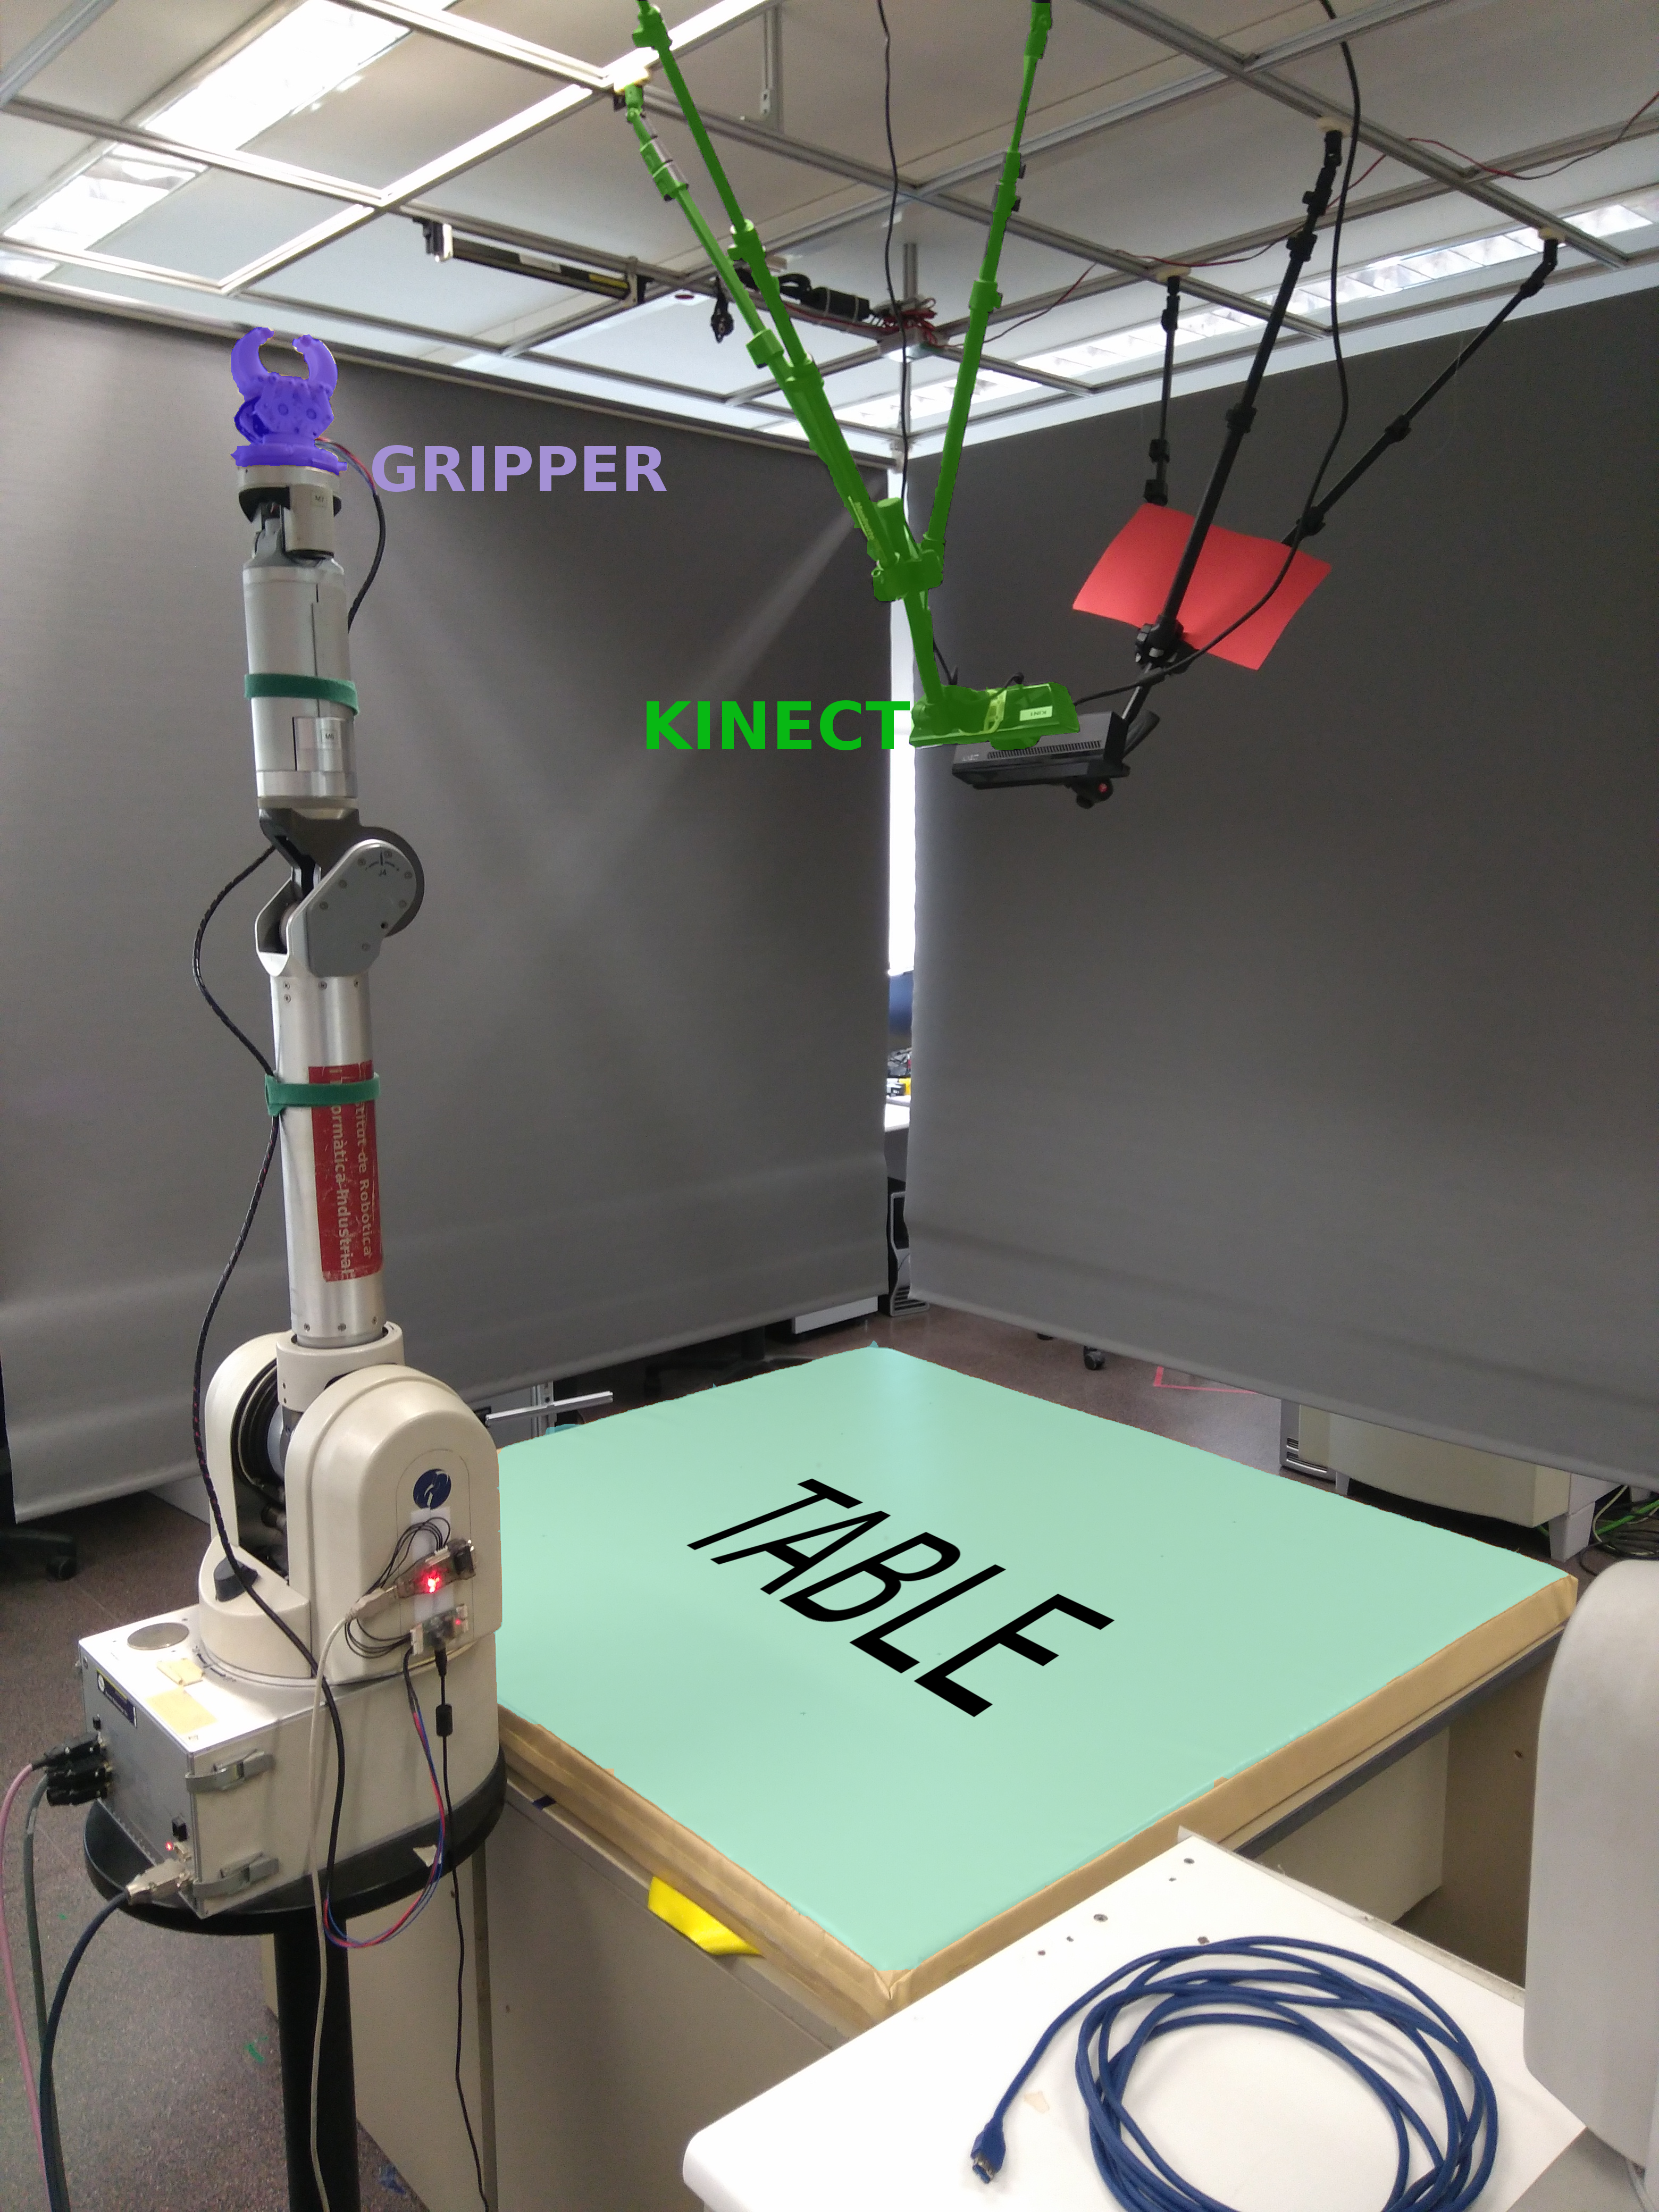
\includegraphics[width=0.5\textwidth]{Img/set_up/set_up_nice.png}
\caption{Principal elements of the experimental set up.}\label{fig:setup}
\end{figure}